\documentclass[a4paper,12pt]{article}

\usepackage{graphicx, amsmath, amsfonts, amsthm, fullpage, enumitem, calc, hyperref}

\newcommand{\ie}{i.e.}
\newcommand{\Holder}{H\"{o}lder}
\newcommand{\realR}{\mathbb{R}}
\newcommand{\ratQ}{\mathbb{Q}}
\newcommand{\intZ}{\mathbb{Z}}

\newtheorem{thm}{Theorem}[section]
\newtheorem{prop}[thm]{Proposition}
\newtheorem{cor}[thm]{Corollary}

\theoremstyle{definition}
\newtheorem{defn}[thm]{Definition}
\newtheorem{expl}[thm]{Example}

\theoremstyle{remark}
\newtheorem{rmk}[thm]{Remark}

\DeclareMathOperator{\const}{const}

\title{Lecture notes of MA3209: Metric space}
\author{WANG Dong}

\begin{document}

\maketitle

New topics will be added to the notes after each class, and typos will be fixed anytime they are spotted.

\section{Definition and examples of metric spaces}

\begin{defn}
  A \emph{metric space} $R = (X, \rho)$ is the pair of two things: a set $X$, whose elements are called points, and a distance, \ie, a single-valued, nonnegative real function $\rho(x,y)$, defined for arbitrary $x$ and $y$ in $X$, such that
  \begin{enumerate}
  \item \label{enu:metric_1}
    $\rho(x,y) = 0$ if and only if $x = y$,
  \item \label{enu:metric_2}
    $\rho(x,y) = \rho(y,x)$ (axiom of symmetry),
  \item \label{enu:metric_3}
    $\rho(x,y) + \rho(y,z) \geq (x,z)$ (triangle axiom).
  \end{enumerate}
\end{defn}

\begin{expl}
  $X = \realR$ and $\rho(x,y) = \lvert x-y \rvert$.
\end{expl}

\begin{expl} \label{expl:Euclidean}
  (Euclidean $n$-space) $X = \realR^n$ and for $x = (x_1, x_2, \dotsc, x_n)$, $y = (y_1, y_2, \dotsc, y_n)$,
  \begin{equation*}
  \rho(x, y) = \sqrt{(x_1 - y_1)^2 + (x_2 - y_2)^2 + \dotsb + (x_n - y_n)^2}.
  \end{equation*}
\end{expl}

\begin{figure}[h]
  \centering
  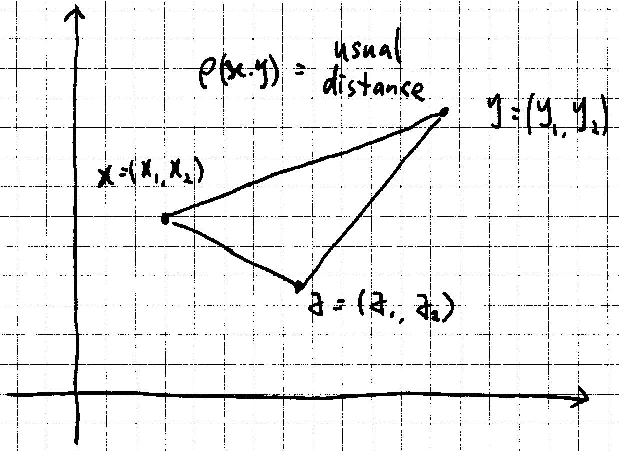
\includegraphics{fig1}
  \caption{When $n = 2$, we see from the figure that $\rho(x,y)$ is the usual distance and the triangle axiom has a simple geometric meaning.}
\end{figure}
In that space, conditions \ref{enu:metric_1} and \ref{enu:metric_2} are obviously satisfied. To validate condition \ref{enu:metric_3}, we denote
\begin{align*}
  a = {}& (a_1, a_2, \dotsc, a_n) = (x_1 - y_1, x_2 - y_2, \dotsc, x_n - y_n), \\
  b = {}& (b_1, b_2, \dotsc, b_n) = (y_1 - z_1, y_2 - z_2, \dotsc, y_n - z_n).
\end{align*}
then
\begin{align*}
  & \rho(x,z) \leq \rho(x,y) + \rho(y,z) \\
  \Longleftrightarrow {}& \sqrt{(a_1 + b_1)^2 + \dotsc + (a_n + b_n)^2} \leq \sqrt{a^2_1 + \dotsc + a^2_n} + \sqrt{b^2_1 + \dotsc + b^2_n} \\
  \Longleftrightarrow {}& (a_1 + b_1)^2 + \dotsc + (a_n + b_n)^2 \\
  & \leq (a^2_1 + \dotsc + a^2_n) + (b^2_1 + \dotsc + b^2_n) + 2 \sqrt{a^2_1 + \dotsc + a^2_n} \sqrt{b^2_1 + \dotsc + b^2_n} \\
  \Longleftrightarrow {}& 2(a_1b_1 + a_2b_2 + \dotsc + a_nb_n) \leq 2 \sqrt{a^2_1 + \dotsc + a^2_n} \sqrt{b^2_1 + \dotsc + b^2_n}.
\end{align*}
Then it is a consequence of the following theorem.
\begin{thm}[Schwarz inequality]
  For all real numbers $a_1, a_2, \dotsc, a_n$ and $b_1, b_2, \dotsc, b_n$,
  \begin{equation} \label{eq:Schwarz}
    (a_1b_1 + a_2b_2 + \dotsc + a_nb_n)^2 \leq (a^2_1 + a^2_2 + \dotsc + a^2_n) (b^2_1 + b^2_2 + \dotsc + b^2_n).
  \end{equation}
\end{thm}
\begin{proof}
  The right-hand side of \eqref{eq:Schwarz} can be expanded as
  \begin{equation*}
    \begin{split}
      (a^2_1 + a^2_2 + \dotsc + a^2_n) (b^2_1 + b^2_2 + \dotsc + b^2_n) ={}& \sum^n_{i=1} \sum^n_{j=1} a^2_i b^2_j = \sum^n_{i=1} \sum^n_{j=1} a^2_j b^2_i \\
      ={}& \frac{1}{2} \sum^n_{i=1} \sum^n_{j=1} a^2_i b^2_j + a^2_j b^2_i.
    \end{split}
  \end{equation*}
On the other hand, the left-hand side of \eqref{eq:Schwarz} can be expanded as
\begin{equation*}
  (a_1b_1 + a_2b_2 + \dotsc + a_nb_n)^2 = \sum^n_{i=1} \sum^n_{j=1} (a_ib_i)(a_jb_j) = \frac{1}{2} \sum^n_{i=1} \sum^n_{j=1} 2(a_ib_j)(a_jb_i).
\end{equation*}
Thus we have
\begin{equation*}
  (a^2_1 + a^2_2 + \dotsc + a^2_n) (b^2_1 + b^2_2 + \dotsc + b^2_n) - (a_1b_1 + a_2b_2 + \dotsc + a_nb_n)^2 = \frac{1}{2} \sum^n_{i=1} \sum^n_{j=1} (a_ib_j - a_jb_i)^2 \geq 0,
\end{equation*}
and finish the proof.
\end{proof}

\begin{expl}
  $X = \realR^n$ and
  \begin{equation*}
    \rho_p(x,y) = \left( \lvert x_1 - y_1 \rvert^p + \lvert x_2 - y_2 \rvert^p + \dotsc + \lvert x_n - y_n \rvert^p \right)^{\frac{1}{p}}.
  \end{equation*}
\end{expl}
In this example, conditions \ref{enu:metric_1} and \ref{enu:metric_2} are obviously satisfied, and condition \ref{enu:metric_3}, based on arguments similar to those in the for Example \ref{expl:Euclidean}, is equivalent to the following theorem.
\begin{thm}[Minkowski inequality]
  For all real numbers $a_1, a_2, \dotsc, a_n$, $b_1, b_2, \dotsc, b_n$, and $p \geq 1$,
  \begin{equation*}
    (\lvert a_1 + b_1 \rvert^p + \dotsc + \lvert a_n + b_n \rvert^p)^{\frac{1}{p}} \leq (\lvert a_1 \rvert^p + \dotsc + \lvert a_1 \rvert^p)^{\frac{1}{p}} + (\lvert b_1 \rvert^p + \dotsc + \lvert b_1 \rvert^p)^{\frac{1}{p}}.
  \end{equation*}
\end{thm}
The proof of the Minkowski inequality when $p > 1$ depends on \Holder's inequality, while the $p = 1$ case turns out to be much easier.

\begin{thm}[\Holder's inequality]
  For all real numbers $x_1, x_2, \dotsc, x_n$, $y_1, y_2, \dotsc, y_n$, and $p, q > 1$ such that $\frac{1}{p} + \frac{1}{q} = 1$,
  \begin{equation*}
    \sum^n_{k=1} \lvert x_k y_k \rvert \leq \left( \sum^n_{k=1} \lvert x_k \rvert^p \right)^{\frac{1}{p}}  \left( \sum^n_{k=1} \lvert y_k \rvert^q \right)^{\frac{1}{q}}.
  \end{equation*}
\end{thm}
\begin{proof}[Proof of the Minkowski inequality ($p > 1$) from \Holder's inequality]
  We starts from a simple identity
  \begin{equation} \label{simple_id_for_Holder}
    (\lvert a \rvert + \lvert b \rvert)^p = \lvert a \rvert (\lvert a \rvert + \lvert b \rvert)^{p-1} + \lvert b \rvert (\lvert a \rvert + \lvert b \rvert)^{p-1}.
  \end{equation}
  By \Holder's inequality,
  \begin{equation*}
    \begin{split}
      \sum^n_{k=1} \lvert a_k \rvert (\lvert a_k \rvert + \lvert b_k \rvert)^{p-1} \leq {}& \left( \sum^n_{k=1} \lvert a_k \rvert^p \right)^{\frac{1}{p}} \left( \sum^n_{k=1} \left[ (\lvert a_k \rvert + \lvert b_k \rvert)^{p-1} \right]^q \right)^{\frac{1}{q}} \\
      = {}& \left( \sum^n_{k=1} \lvert a_k \rvert^p \right)^{\frac{1}{p}} \left( \sum^n_{k=1} (\lvert a_k \rvert + \lvert b_k \rvert)^p \right)^{1 - \frac{1}{p}},
    \end{split}
  \end{equation*}
  where we use the relation $q = \frac{p}{p-1}$ in the last step. Similarly,
  \begin{equation*}
    \begin{split}
      \sum^n_{k=1} \lvert b_k \rvert (\lvert a_k \rvert + \lvert b_k \rvert)^{p-1} \leq {}& \left( \sum^n_{k=1} \lvert b_k \rvert^p \right)^{\frac{1}{p}} \left( \sum^n_{k=1} \left[ (\lvert a_k \rvert + \lvert b_k \rvert)^{p-1} \right]^q \right)^{\frac{1}{q}} \\
      = {}& \left( \sum^n_{k=1} \lvert b_k \rvert^p \right)^{\frac{1}{p}} \left( \sum^n_{k=1} (\lvert a_k \rvert + \lvert b_k \rvert)^p \right)^{1 - \frac{1}{p}}.
    \end{split}
  \end{equation*}
Sum up the two identities above, we obtain with the help of the simple identity \eqref{simple_id_for_Holder}
\begin{equation*}
  \sum^n_{k=1} (\lvert a_k \rvert + \lvert b_k \rvert)^p \leq \left[ \left( \sum^n_{k=1} \lvert a_k \rvert^p \right)^{\frac{1}{p}} + \left( \sum^n_{k=1} \lvert b_k \rvert^p \right)^{\frac{1}{p}} \right] \left( \sum^n_{k=1} (\lvert a_k \rvert + \lvert b_k \rvert)^p \right)^{1 - \frac{1}{p}}.
\end{equation*}
Dividing $\left( \sum^n_{k=1} (\lvert a_k \rvert + \lvert b_k \rvert)^p \right)^{1 - \frac{1}{p}}$ on both sides, we prove the Minkowski inequality.
\end{proof}

\begin{proof}[Proof of \Holder's inequality]
  First we show a short inequality
  \begin{equation} \label{eq:short_ineq_for_Holder}
    ab \leq \frac{a^p}{p} + \frac{b^q}{q},
  \end{equation}
  for $a, b > 0$, $p, q > 1$ and $\frac{1}{p} + \frac{1}{q} = 1$. The proof of the inequality relies on the integral formula
  \begin{align*}
    \frac{a^p}{p} = {}& \int^a_0 x^{p-1} dx, \\
    \frac{b^q}{q} = {}& \int^b_0 y^{q-1} dy = \int^b_0 y^{\frac{1}{p-1}} dy,
  \end{align*}
  where in the second formula we used the relation $q-1 = \frac{1}{p-1}$ as a consequence of $\frac{1}{p} + \frac{1}{q} = 1$. Hence $\frac{a^p}{p}$ and $\frac{b^q}{q}$ are expressed geometrically as the following areas of regions.
  \begin{figure}[h]
    \centering
    \begin{minipage}{0.49\linewidth}
      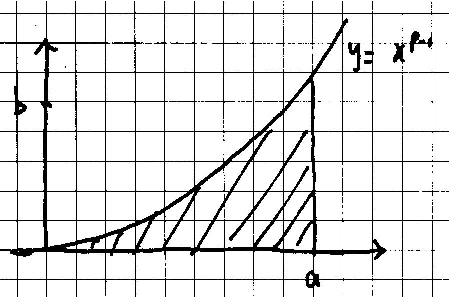
\includegraphics{a_to_p}
    \end{minipage}
    \begin{minipage}{0.49\linewidth}
      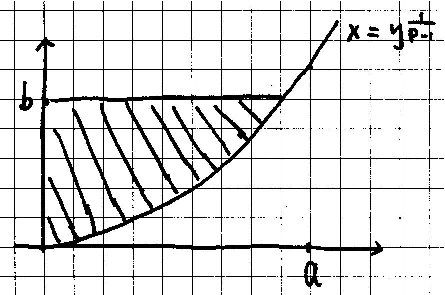
\includegraphics{b_to_q}
    \end{minipage}
    \caption{The areas of the two shaded regions represent $\frac{a^p}{p}$ and $\frac{b^q}{q}$ respectively.}
  \end{figure}

  Noting that the graph of $x = y^{\frac{1}{p-1}}$ coincides with that of $y = x^{p-1}$, we put the two graphs in one figure:

  Then it is clear that $ab$, geometrically represented by the area of the rectangle, is smaller than the sum of $\frac{a^p}{p}$ and $\frac{b^q}{q}$ by a ``corner'', see Figure \ref{fig:small_b_value}.
  \begin{figure}[h]
    \centering
    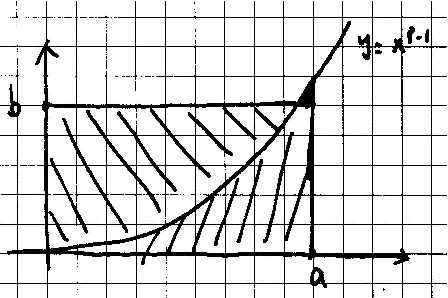
\includegraphics{small_b_value}
    \label{fig:small_b_value}
    \caption{$\frac{a^p} + \frac{b^q}{q}$ is larger than $ab$ by the area of the area of the solid coner.}
  \end{figure}
  If the value of $b$ is larger, the ``corner'' occurs in a different place, see Figure \ref{fig:large_b_value}.
  \begin{figure}[h]
    \centering
    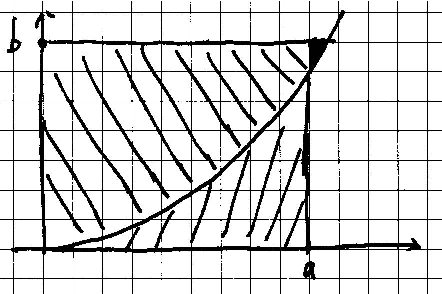
\includegraphics{large_b_value}
    \label{fig:large_b_value}
    \caption{$\frac{a^p}{p} + \frac{b^q}{q}$ is larger than $ab$ by the area of the area of the solid coner.}
  \end{figure}
  
  Note that \Holder's inequality is \emph{homogeneous}, in the sense that if it holds for $x = (x_1, \dotsc, x_n)$ and $y = (y_1, \dotsc, y_n)$, then it also holds for $\lambda x = (\lambda x_1, \dotsc, \lambda x_n)$ and $\mu y = (\mu y_1, \dotsc, \mu y_n)$:
  \begin{equation*}
    \begin{split}
      & \sum^n_{k=1} \lvert x_k y_k \rvert \leq \left( \sum^n_{k=1} \lvert x_k \rvert^p \right)^{\frac{1}{p}}  \left( \sum^n_{k=1} \lvert y_k \rvert^q \right)^{\frac{1}{q}} \\
      \Longleftrightarrow {}& \sum^n_{k=1} \lvert \lambda x_k \mu y_k \rvert \leq \left( \sum^n_{k=1} \lvert \lambda x_k \rvert^p \right)^{\frac{1}{p}}  \left( \sum^n_{k=1} \lvert \mu y_k \rvert^q \right)^{\frac{1}{q}}.
    \end{split}
  \end{equation*}
Thus we need only to prove it under the condition $\sum^n_{k=1} \lvert x_k \rvert^p = 1$ and $\sum^n_{k=1} \lvert y_k \rvert^q = 1$. In that case, the short inequality \eqref{eq:short_ineq_for_Holder} implies that for each $k$, $\lvert x_k y_k \rvert \leq \frac{\lvert x_k \rvert^p}{p} + \frac{\lvert y_k \rvert^q}{q}$. Sum up for $k$ from $1$ to $n$, we have
\begin{equation*}
  \begin{split}
    \sum^n_{k=1} \lvert x_k y_k \rvert \leq {}& \sum^n_{k=1} \frac{\lvert x_k \rvert^p}{p} + \frac{\lvert y_k \rvert^q}{q} = \frac{1}{p}\sum^n_{k=1} \lvert x_k \rvert^p + \frac{1}{q}\sum^n_{k=1} \lvert y_k \rvert^q = \frac{1}{p} + \frac{1}{q} \\
    & = 1 = \left( \sum^n_{k=1} \lvert x_k \rvert^p \right)^{\frac{1}{p}}  \left( \sum^n_{k=1} \lvert y_k \rvert^q \right)^{\frac{1}{q}},
  \end{split}
\end{equation*}
and prove the special case. The theorem in general setting is then proved by the homogeneous property.
\end{proof}

\begin{expl} \label{expl:rho_infty_R^n}
  $X = \realR^n$ and $\rho(x,y) = \max^n_{k=1}(\lvert x_k - y_k \rvert)$.
\end{expl}
The verification that the space is a metric space is left as an exercise.
\begin{rmk}
  The distance in Euclidean $n$-space is $\rho_2$, and the distance in Example \ref{expl:rho_infty_R^n} is, in some sense, the limit of $\rho_p$ as $p \to \infty$:
  \begin{equation*}
    \rho_{\infty}(x, y) = \lim_{p \to \infty} \rho_p(x, y), \quad \text{for all $x, y \in \realR^n$.}
  \end{equation*}
  The proof of the above limit identity is left for exercise.
\end{rmk}

\begin{expl}[$\ell^p$ space]
  $X$ is the set of all possible sequences $x = (x_1, x_2, \dotsc, x_n, \dotsc)$ of real numbers, which satisfies the condition $\sum^{\infty}_{k=1} \lvert x_k \rvert^p < \infty$. The distance function is ($p \geq 1$)
  \begin{equation*}
    \rho_p(x, y) = \left( \sum^{\infty}_{k=1} \lvert x_k - y_k \rvert^p \right)^{\frac{1}{p}}.
  \end{equation*}
\end{expl}

First we show that $\rho_p(x, y)$ is well defined. For any $n$,
\begin{equation*}
  \begin{split}
    \left( \sum^n_{k=1} \lvert x_k - y_k \rvert^p \right)^{\frac{1}{p}} \leq {}& \left( \sum^n_{k=1} \lvert x_k \rvert^p \right)^{\frac{1}{p}} + \left( \sum^n_{k=1} \lvert y_k \rvert^p \right)^{\frac{1}{p}} \\
    \leq {}& \left( \sum^{\infty}_{k=1} \lvert x_k \rvert^p \right)^{\frac{1}{p}} + \left( \sum^{\infty}_{k=1} \lvert y_k \rvert^p \right)^{\frac{1}{p}} = \const < \infty,
  \end{split}
\end{equation*}
where in the first step we use the Minkowski inequality. Since $\left( \sum^n_{k=1} \lvert x_k - y_k \rvert^p \right)^{\frac{1}{p}}$ increases monotonically as $n \to \infty$, the limit exists by the \emph{monotone convergence theorem}, and it is $\rho_p(x,y)$.

Then we show the condition \ref{enu:metric_3} holds, that is,
\begin{equation*}
  \left( \sum^{\infty}_{k=1} \lvert x_k - z_k \rvert^p \right)^{\frac{1}{p}} - \left[ \left( \sum^{\infty}_{k=1} \lvert x_k - y_k \rvert^p \right)^{\frac{1}{p}} + \left( \sum^{\infty}_{k=1} \lvert y_k - z_k \rvert^p \right)^{\frac{1}{p}} \right] \leq 0.
\end{equation*}
This is the $n \to \infty$ limit of the inequality
\begin{equation*}
  \left( \sum^n_{k=1} \lvert x_k - z_k \rvert^p \right)^{\frac{1}{p}} - \left[ \left( \sum^n_{k=1} \lvert x_k - y_k \rvert^p \right)^{\frac{1}{p}} + \left( \sum^n_{k=1} \lvert y_k - z_k \rvert^p \right)^{\frac{1}{p}} \right] \leq 0.
\end{equation*}

\begin{expl}[$\ell^{\infty}$ space]
  $X$ is the set of all possible sequences $x = (x_1, x_2, \dotsc, x_n, \dotsc)$ of real numbers, which satisfies the condition $\sup^{\infty}_{k=1} \lvert x_k - y_k \rvert$. The distance function is
  \begin{equation*}
    \rho_p(x) = \sup^{\infty}_{k=1} \lvert x_k - y_k \rvert.
  \end{equation*}
\end{expl}

\begin{expl}[{$C^p([a, b])$ space}]
  $X$ is the set of all continuous functions on interval $[a, b]$. The distance is ($p \geq 1$)
  \begin{equation*}
    \rho_p(x, y) = \left( \int^b_a \lvert x(t) - y(t) \rvert^p \right)^{\frac{1}{p}}.
  \end{equation*}
\end{expl}

The distance function $\rho_p(x, y)$ is well defined since $x(t)$ and $y(t)$ are bounded, which is a consequence of the extreme value theorem. To show condition \ref{enu:metric_3} holds, we need the integral form of the Minkowski inequality. The proof is a homework problem.

\begin{expl}[{$C^{\infty}  ([a, b ]) $ space}]
  $X$ is the set of all continuous functions on interval $[a, b]$. The distance is
  \begin{equation*}
    \rho_{\infty}(x, y) = \max_{t \in [a, b]} (\lvert x(t) - y(t) \rvert).
  \end{equation*}
\end{expl}

It is an exercise to show that the distance function $\rho_{\infty}(x, y)$ satisfies the triangle axiom (condition \ref{enu:metric_3}).

\section{Convergence of sequences. Limit points}

\begin{defn}
  An \emph{open ball} $B(x_0, r)$ in the metric space $R$ is the set of all points $x$ in $R$ which satisfy the condition $\rho(x, x_0) < r$. $x_0$ is called the \emph{centre} and $r$ the \emph{radius}. The open ball is also called a \emph{neighbourhood} of $x_0$, denoted as $N_r(x_0)$.
\end{defn}
\begin{expl}
  The open balls in $\realR^2$ with origin as their center and radius $1$, in metric spaces with distance function $\rho_1$, $\rho_2$ (Euclidean $2$-space), $\rho_4$ and $\rho_{\infty}$ are shown below.
  \begin{figure}[h]
    \centering
    \begin{minipage}[t]{0.24\linewidth}
      \includegraphics{open_ball_1}
    \end{minipage}
    \begin{minipage}[t]{0.24\linewidth}
      \includegraphics{open_ball_2}
    \end{minipage}
    \begin{minipage}[t]{0.24\linewidth}
      \includegraphics{open_ball_3}
    \end{minipage}
    \begin{minipage}[t]{0.24\linewidth}
      \includegraphics{open_ball_4}
    \end{minipage}
    \caption{The open balls with center $(0,0)$ and radius $1$ in $(\realR^2, \rho_1)$, $(\realR^2, \rho_2)$, $(\realR^2, \rho_4)$ and $(\realR^2, \rho_{\infty})$ respectively.}
  \end{figure}
\end{expl}

\begin{defn}
  A \emph{closed ball} $B[x_0, r]$ is the set of all points $x$ in $R$ which satisfy the condition $\rho(x, x_0) \leq r$.
\end{defn}
\begin{expl}
  The closed balls in $\realR^2$ with origin as their center and radius $1$, in metric spaces with distance function $\rho_1$, $\rho_2$ (Euclidean $2$-space), $\rho_4$ and $\rho_{\infty}$ are shown below.
  \begin{figure}[h]
    \centering
    \begin{minipage}[t]{0.24\linewidth}
      \includegraphics{closed_ball_1}
    \end{minipage}
    \begin{minipage}[t]{0.24\linewidth}
      \includegraphics{closed_ball_2}
    \end{minipage}
    \begin{minipage}[t]{0.24\linewidth}
      \includegraphics{closed_ball_3}
    \end{minipage}
    \begin{minipage}[t]{0.24\linewidth}
      \includegraphics{closed_ball_4}
    \end{minipage}
    \caption{The closed balls with center $(0,0)$ and radius $1$ in $(\realR^2, \rho_1)$, $(\realR^2, \rho_2)$, $(\realR^2, \rho_4)$ and $(\realR^2, \rho_{\infty})$ respectively.}
  \end{figure}
\end{expl}

\begin{defn}
  A point $x$ is called a \emph{contact point} of the set $M$ if every neighbourhood of $x$ contains at least one point of $M$. The set of all contact points of the set $M$ is the \emph{closure} of $M$, denoted by $\overline{M}$.
\end{defn}

In last example, the closure of $B((0,0), 1)$, the open ball, is the closed ball $B[(0,0), 1]$. See the figure below for an explanation in the Euclidean $2$-space, and other cases are left for exercise.
\begin{figure}[h]
  \centering
  \includegraphics{open_ball_closure}
  \caption{The point $x_1$, in the open ball, is in the closure of the open ball since all its neighbourhoods at least contains itself; the point $x_2$, outside of the closed ball, is not in the closure of the open ball since it has a small neighbourhood disjoint to the open ball; the point $x_3$, lying on the boundary of the ball, is in the closure, since all its neibourhoods, however small, intersect with the open ball.}
\end{figure}

However, is the closure of the open ball $B(x_0, r)$ the closed ball $B[x_0, r]$ in \emph{all} matric spaces? The answer is NO, and we have a counterexample as follows.
\begin{expl}[discrete metric space]
  Let $X$ be any set (of more than one element), and
  \begin{equation*}
    \rho(x, y) =
    \begin{cases}
      1 & \text{if $x \neq y$,} \\
      0 & \text{if $x = y$.}
    \end{cases}
  \end{equation*}
  Then for any $x$ in $X$, $B(x, 1) = \{ x \}$, and $B[x, 1] = X$. Since for any $y \neq x$, $x \not\in N_{\frac{1}{2}}(y)$, we have $\overline{B(x, 1)} = \{ x \}$, and then $\overline{B(x, 1)} \neq B[x, 1]$.
\end{expl}

\begin{thm}
  The closure of the closure of $M$ is equal to the closure of $M$: $\overline{\overline{M}} = \overline{M}$.
\end{thm}
\begin{proof}
  Every point of $M$ is a contact point of $M$, so $\overline{M} \supseteq M$, and also $\overline{\overline{M}} \supseteq \overline{M}$. Then we need to show that if $x \in \overline{\overline{M}}$, it is also in $\overline{M}$. If $x$ is in $\overline{\overline{M}}$ but not in $\overline{M}$, there exists a neighbourhood $N_{\epsilon}(x)$ of $x$ such that it does not intersect with $M$. Since $x \in \overline{\overline{M}}$, $N_{\frac{\epsilon}{3}}(x)$ contains a point $x_1$ in $\overline{M}$. Then the neighbourhood $N_{\frac{\epsilon}{3}}(x_1)$ of $x_1$ contains a point $x_2$ in $M$ since $x_1 \in \overline{M}$. By the triangle inequality,
  \begin{equation*}
    \rho(x, x_2) \leq \rho(x, x_1) + \rho(x_1, x_2) < \frac{\epsilon}{3} + \frac{\epsilon}{3} = \frac{2}{3}\epsilon < \epsilon,
  \end{equation*}
  which is contradictory to the assumption that $N_{\epsilon}(x)$ does not intersect with $M$.
\end{proof}

\begin{thm}
  If $M_1 \subseteq M_2$, then $\overline{M_1} \subseteq \overline{M_2}$.
\end{thm}
\begin{proof}
  Exercise.
\end{proof}

\begin{thm} \label{thm:closure_sum}
  The closure of a sum is equal to the sum of clusures: $\overline{M_1 \cup M_2} = \overline{M_1} \cup \overline{M_2}$.
\end{thm}
\begin{proof}
  Be Theorem \ref{thm:closure_sum}, $\overline{M_1 \cup M_2} \supseteq \overline{M_1}$ since $M_1 \cup M_2 \supseteq M_1$, and similarly $\overline{M_1 \cup M_2} \supseteq \overline{M_2}$. Thus $\overline{M_1 \cup M_2} \supseteq \overline{M_1} \cup \overline{M_2}$.

  Now we show that $\overline{M_1 \cup M_2} \subseteq \overline{M_1} \cup \overline{M_2}$. If there exists $x$ in $\overline{M_1 \cup M_2}$ but not in $\overline{M_1} \cup \overline{M_2}$, then there exists $N_{\epsilon_1}(x)$ that is disjoint to $M_1$, and $N_{\epsilon_2}(x)$ that is disjoint to $M_2$. We have $N_{\min(\epsilon_1, \epsilon_2)}(x)$, the intersection between the two neighbourhood, is disjoint to both $M_1$ and $M_2$, which means $N_{\min(\epsilon_1, \epsilon_2)}(x) \cap (M_1 \cup M_2) = \emptyset$. This is contradictory to the assumption that $x \in \overline{M_1 \cup M_2}$.
\end{proof}

\begin{defn}
  The point $x$ is called a \emph{limit point} of the set $M$ if an arbitrary neighbourhood of $x$ contains an infinite number of points of $M$, and is called an \emph{isolated point} of $M$ if $x$ is in $M$ and has a neighbourhood $N_{\delta}(x)$ that does not contain any point of $M$ different from $x$.
\end{defn}

\begin{thm}
  Every contact point of the set $M$ is either a limit point or an isolated point of $M$.
\end{thm}
\begin{proof}
  Let $x$ be a contact point of $M$, but not a limit point. Then there is a neighbourhood $N_{\epsilon}(x)$ such that it contains only finitely many points $x_1, x_2, \dotsc, x_k$ in $M$. Let $\rho(x, x_i) = \epsilon_i$ for $i = 1, 2, \dotsc, k$, and take $\bar{\epsilon}$ be the smallest one among nonzero values of $\epsilon_i$. (One of $\epsilon_i$ may be $0$, which means that $x$ itself is among the $k$ points.) Then the neighbourhood $N_{\bar{\epsilon}}(x)$ contains no points among $x_1, \dotsc, x_k$ that are different from $x$, in other words, it contains no points in $M$ that are different from $x$. We conclude that $x$ is an isolated point of $M$.
\end{proof}
\begin{rmk}
  As a conclusion of the proof, we see that the point $x$ is in $M$. But in the intermediate steps, this fact is not clear at all, and we cannot make use of it.
\end{rmk}

Thus the closure of a set can be divided into
\begin{multline*}
  \overline{M} = \{ \text{isolated points} \} \cup \{ \text{limit points that belong to $M$} \} \\
  \cup \{ \text{limit points that does not belong to $M$} \}.
\end{multline*}

\begin{defn}
  Let $x_1, x_2, \dotsc$ be a sequence of points in the metric space $R$, we say this sequence \emph{converges to } the point $x$ if every neighbourhood $N_{\epsilon}(x)$ contains all points $x_n$ starting with some one of them. The point $x$ is called the \emph{limit} of the sequence $\{ x_n \}$.
\end{defn}

Two simple properties:
\begin{itemize}
\item No sequence can have two distinct limits.
\item If $\{ x_n \}$ converges to $x$, so does any of its subsequence.
\end{itemize}

\begin{thm} \label{thm:contact_limit_and_sequence}
  \begin{itemize}
  \item The point $x$ is a contact point of the set $M$ if and only if there exists a sequence $\{ x_n \}$ of points of the set $M$ which converges to $x$.
  \item The point $x$ is a limit point of $M$ if and only if there exists a sequence $\{ x_n \}$ of \emph{distinct} points of the set $M$ which converges to $x$.
  \end{itemize}
\end{thm}
\begin{proof}
  If $\{ x_n \} \subset M$ converges to $x$, then in any neighbourhood $N_{\epsilon}(x)$ there are points $\{ x_n, x_{n+1}, x_{n+2}, \dotsc \} \subset M$ lying in $N_{\epsilon}(x)$. (Here $n$ depends on $\epsilon$). So $x$ is a contact point. Furthermore, if $\{ x_n, x_{n+1}, \dotsc \}$ are distinct points, then $N_{\epsilon}(x)$ contains infinitely many points of $M$, and it is a limit point.

  Conversely, if $x$ is a contact point of $M$, then we construct $x_1, x_2, \dotsc$ as follows:
  \begin{itemize}[labelindent= \widthof{Step $n$}, leftmargin=*]
  \item[Step $1$:]
    Choose $x_1$ as a point in $M$ that lies in $N_{\frac{1}{1}}(x)$.
  \item[Step $2$:]
    Choose $x_2$ as a point in $M$ that lies in $N_{\frac{1}{2}}(x)$.

    $\ldots$ $\ldots$
    
  \item[Step $n$:]
    Choose $x_n$ as a point in $M$ that lies in $N_{\frac{1}{n}}(x)$.

    $\ldots$ $\ldots$
    
  \end{itemize}
  and we construct the desired sequence in $M$ that converges to $x$. If $x$ is further a limit point, in Step $n$ ($n > 1$) we ``choose $x_n$ as a point in $M$ that lies in $N_{\frac{1}{n}}(x)$ that is \emph{distinct} from $x_1, x_2, \dotsc, x_{n-1}$. 
\end{proof}

\begin{defn}
  Let $A$ and $B$ be two sets in the metric cpace $R$. The set $A$ is \emph{dense} in $B$ if $\overline{A} \supseteq B$, In particular, $A$ is \emph{everywhere dense} if $\overline{A} = R$.
\end{defn}

\begin{defn}
  The metric space $R$ is \emph{separable} if it has an everywhere dense subset that is countable.
\end{defn}

\begin{expl} \label{expl:R_is_separable}
  The metric space $R = (\realR, \rho(x, y) = \lvert x - y \rvert)$ is separable, and the countable set of rational numbers is everywhere dense.
\end{expl}
\begin{proof}
  For any real number $x$, let $x_n$ be the largest rational number in the form $\frac{m}{10^n}$ ($m$ is an integer) that is less than or equal to $x$. Then $\{ x_1, x_2, \dotsc \}$ converges to $x$. By Theorem \ref{thm:contact_limit_and_sequence}, $x$ is a contact point of $\ratQ = \{ \text{rational numbers} \}$, and $\ratQ$ is everywhere dense.

  One example of the construction: if $x = \pi$, then $x_1 = \frac{31}{10^1} = 3.1$, $x_2 = \frac{314}{10^2} = 3.14$, $x_3 = \frac{3141}{10^3} = 3.141$, \dots.
\end{proof}

\begin{expl}
  The metric space $R = (\realR^m, \rho_{\infty}(x, y) = \max^n_{k=1}( \lvert x_k - y_k \rvert ))$ is separable, and the countable set $A = \{ x = (x_1, x_2, \dotsc, x_m) : x_k \in \ratQ \}$ is everywhere dense. 
\end{expl}
\begin{proof}
  For any point $\bar{x} = (\bar{x}_1, \dotsc, \bar{x}_m)$, let the sequence $\{ x^{(n)}_k \}$ be the sequence constructed in Example \ref{expl:R_is_separable}. Then as $n \to \infty$, $x^{(n)} = (x^{(n)}_1, x^{(n)}_2, \dotsc, x^{(n)}_m)$ converges to $\bar{x}$.
\end{proof}

\begin{expl}
  $\ell^{\infty}$ space is not separable.
\end{expl}
  To show that all everywhere dense subset of $\ell^{\infty}$ space are uncountable, we need the fact that
  \begin{prop} \label{prop:Cantor_theorem}
    The subsets of the set of all positive integers ($\intZ_+ = \{ 1, 2, 3, \dotsc \}$) is an uncountable set.
  \end{prop}
  The proof of this proposition will be given in Appendix \ref{sec:proof_of_Cantor_theorem}.
\begin{proof}[Proof of that $\ell^{\infty}$ is not separable]
  Let $S$ be any subset of $\intZ_+$. Define $x^{(S)} \in \ell^{\infty}$ as
  \begin{equation*}
    x^{(S)} = (x^{(S)}_1, \dotsc, x^{(S)}_m), \quad \text{where} \quad x^{(S)}_k =
    \begin{cases}
      1 & \text{if $k \in S$,} \\
      0 & \text{if $k \not\in S$.}
    \end{cases}
  \end{equation*}
  Then we see that
  \begin{equation} \label{eq:dist_between_x^S}
    \rho_{\infty}(x^{(S)}, x^{(S')}) =
    \begin{cases}
      1 & \text{if $S \neq S'$,} \\
      0 & \text{if $S = S'$.}
    \end{cases}
  \end{equation}
  Suppose $A$ is an everywhere dense subset of $R$. For each $x^{(S)}$, there is an $a^{(S)} \in A$ lying in $N_{\frac{1}{3}}(x^{(S)})$. The points $a^{(S)}$ are distinct. Otherwise if $a^{(S)} = a^{(S')}$ with $S \neq S'$, then
  \begin{equation*}
    \rho_{\infty}(x^{(S)}, x^{(S')}) \leq \rho_{\infty}(x^{(S)}, a^{(S)}) + \rho_{\infty}(a^{(S)}, x^{(S')}) \leq \frac{1}{3} + \frac{1}{3} = \frac{2}{3},
  \end{equation*}
  which is contradictory to \eqref{eq:dist_between_x^S}.

  This the set $A$ has no less elements than the subsets of $\intZ_+$, and it is an uncountable set.
\end{proof}

\begin{defn}
  Let $x$ be a point in the metric space $R$ and $A$ be a subset of $R$, then the \emph{distance} from $x$ to $A$ is defined as
  \begin{equation*}
    \rho(A, x) = \inf \{ \rho(a, x) : a \in A \}.
  \end{equation*}
  If $A$ and $B$ are subsets of $R$, then the \emph{distance} between $A$ and $B$ is defined as
  \begin{equation*}
    \rho(A, B) = \inf(\rho(a, b) : a \in A, \ b \in B \}.
  \end{equation*}
\end{defn}
We can show that $\rho(A, x) = 0$ if and only if $x$ is a contact point of $A$.

\begin{defn}
  If $A$ is a set in the metric space $R$, then all limit points of $A$ constitute the \emph{derived set} of $A$, denoted by $A'$.
\end{defn}
Unlike the closure of a set, the derived set of a derived set is not the derived set, that is, $(M')' \neq M'$ generally.
\begin{expl}
  In the metric space $R = (\realR, \rho(x, y) = \lvert x - y \rvert)$, $M' = \{ 0 \}$, and $(M')' = \emptyset$. 
\end{expl}

\section{Open and closed sets}

\begin{defn}
  A set $M$ in a metric space $R$ is said to be \emph{closed} if it coincides with its closure: $\overline{M} = M$.
\end{defn}

\begin{expl}
  The closure of any set $M$ is closed, since $\overline{\overline{M}} = \overline{M}$.
\end{expl}

\begin{expl}
  The closed ball $B[x_0, r]$ is a closed set.
\end{expl}
\begin{figure}[h]
  \centering
  \includegraphics{closed_ball_is_closed}
  \caption{The closed ball is closed.}
\end{figure}
\begin{proof}
  It is clear that $B[x_0, r] \subseteq \overline{B[x_0, r]}$. We need to show $B[x_0, r] \supseteq \overline{B[x_0, r]}$. Suppose $x$ is a point not in $B[x_0, r]$, then $\rho(x, x_0) > r$, say, $\rho(x, x_0) = r + \epsilon$ with $\epsilon > 0$. Then the neighbourhood $N_{\frac{\epsilon}{2}}(x)$ contains no points in $B[x_0, r]$. This can be shown by the triangle inequality: if $x'$ is a point in $N_{\frac{\epsilon}{2}}(x)$, then $\rho(x', x_0) \leq r$, and $\rho(x, x_0) \leq \rho(x, x') + \rho(x', x_0) \leq r + \frac{\epsilon}{2}$, which is contradictory to the assumption that $\rho(x, x_0) = r + \epsilon$.

  Thus any point $x$ outside of $B[x_0, r]$ has a neighbourhood that is disjoint to $B[x_0, r]$ and is not a contact point. We prove that $B[x_0, r] \supseteq \overline{B[x_0, r]}$.
\end{proof}

\begin{thm} \label{thm:intersection_and_sum_of_closed_sets}
  The intersection of an arbitrary number of closed sets is a closed set; the sum of a finite number of closed sets is a closed set.
\end{thm}

\begin{proof}
  First, let $\{ M_{\alpha} \}$ be a family of arbitrary number of closed sets. Need to show that if $x$ is not in the intersection $\bigcap_{\alpha} M_{\alpha}$, then $x$ is not a contact point of $\bigcap_{\alpha} M_{\alpha}$, that is, $x$ has a neighbourhood disjoint to it.

  $x$ is not in $\bigcap_{\alpha} M_{\alpha}$ means that $x$ is not in at least one closed set $M_{\alpha}$. Then there exists a neighbourhood $N_{\epsilon}(x)$ that is disjoint to that $M_{\alpha}$. This implies that $N_{\epsilon}(x)$ is disjoint to the intersection $\bigcap_{\alpha} M_{\alpha}$.

  Next we assume $M_1, M_2, \dotsc, M_n$ are closed sets, and need to show that if $x$ is not in the sum of these sets, it has a neighbourhood that is disjoint to the sum. For any $i = 1, 2, \dotsc, n$, since $x$ is outside of the closed set $M_i$, there is a neighbourhood $N_{\epsilon_i}(x)$ that is disjoint to $M_i$. Taking the intersection of these neighbourhoods, which is $N_{\epsilon}(x)$ with $\epsilon = \min(\epsilon_1, \epsilon_2, \dotsc, \epsilon_n)$, then we can verify that $N_{\epsilon}(x)$ is disjoint to the sum $\bigcup^n_{i=1} M_i$.
\end{proof}
You can think why the second part of the proof does not work for infinite sum of closed sets.

\begin{expl}
  The single point set $\{ x_i \}$ is closed (think is as $B[x_i, 0]$). Therefore the finite set $\{x_1, x_2, \dotsc, x_n \}$ is closed, by Theorem \ref{thm:intersection_and_sum_of_closed_sets}. But an arbitrary infinite set is not nesessarily closed. (A good example of a nonclosed countable set is $\ratQ \subset \realR$, with the usual distance function.)
\end{expl}

\begin{defn}
  The point $x$ is said to be an \emph{interior point} of the set $M$ if there exists a neighbourhood $N_{\epsilon}(x)$ of $x$ that is contained in $M$. The set $M$ is called an \emph{open set} if all of its points are interior points.
\end{defn}

\begin{expl}
  Any point in an open ball $B(x_0, r)$ is an interior point of $B(x_0, r)$, so the open ball $B(x_0, r)$ is an open set.
\end{expl}
\begin{figure}[h]
  \centering
  \includegraphics{open_ball_is_open}
  \caption{The open ball is open.}
\end{figure}
\begin{proof}
  Suppose $x$ is a point in $B(x_0, r)$. Then $\rho(x, x_0) < r$, say, $\rho(x, x_0) = r - \epsilon$ with $\epsilon > 0$. Then the neighbourhood $N_{\frac{\epsilon}{2}}(x)$ is contained in $B(x_0, r)$. This can be shown by the triangle inequality: Any point $x'$ in the neighbourhood $N_{\frac{\epsilon}{2}}(x)$ satisfies $\rho(x', x_0) \leq \rho(x', x) + \rho(x, x_0) \leq (r - \epsilon) + \frac{\epsilon}{2} = r - \frac{\epsilon}{2} < r$, so $x'$ is in the open ball. Thus we have shown that any point $x$ in the open ball is an interior point.
\end{proof}

\begin{thm}
  The set $M$ in metric space $R$ is an open set if and only if its complement $R \setminus M$ is a closed set.
\end{thm}

\begin{proof}
  The property that $M$ is open is equivalent to that any point $x$ in $M$ has a neibourhood $N_{\epsilon}(x)$ contained in $M$. A simple rephrase of this statement is that any point $x$ out of $R \setminus M$ has a neighbourhood $N_{\epsilon}(x)$ disjoint to $R \setminus M$. The rephrased statement is equivalent to say $R \setminus M$ is a closed set.

  Since all steps of the argument are equivalency, the argument above proves both the ``if'' and ``only if'' parts.
\end{proof}

\begin{expl}
  The whole space $R$ is both closed and open (think it informally as $B[x_0, \infty]$ and $B(x_0, \infty)$). Thus its complement, the empty set $\emptyset$, is both open and closed.
\end{expl}

\begin{thm} \label{thm:open_closed_relation}
  The sum of an arbitrary number of open sets is an open set; the intersection of a finite number of open sets are open sets.
\end{thm}

\begin{proof}
  A direct proof like that of Theorem \ref{thm:intersection_and_sum_of_closed_sets} is not very hard and is left as an exercise. Below we show a proof that relies on the result of Theorem \ref{thm:intersection_and_sum_of_closed_sets}.

  We use the identities
  \begin{equation*}
    R \setminus \left( \bigcup_{\alpha} M_{\alpha} \right) = \bigcap_{\alpha} (R \setminus M_{\alpha}), \quad R \setminus \left( \bigcap^n_{i=1} M_i \right) = \bigcap^n_{i=1} (R \setminus M_i).
  \end{equation*}
  
  The statement that $\{ M_{\alpha} \}$ are open sets is equivalent to that $\{ R \setminus M_{\alpha} \}$ are closed sets (Theorem \ref{thm:open_closed_relation}). Then by Theorem \ref{thm:intersection_and_sum_of_closed_sets}, the intersection $\bigcap_{\alpha} (R \setminus M_{\alpha}) = R \setminus \left( \bigcup_{\alpha} M_{\alpha} \right)$ is closed, which implies by Theorem \ref{thm:open_closed_relation} again that $\bigcup_{\alpha} M_{\alpha}$ is open.

  The proof of the latter part of the theorem is similar. The statement that $\{ M_i \}$ are open sets is equivalent to that $\{ R \setminus M_i \}$ are closed sets. Then by Theorem \ref{thm:intersection_and_sum_of_closed_sets}, the sum $\bigcup^n_{i=1} (R \setminus M_i) = R \setminus \left( \bigcap^n_{i=1} M_i \right)$ is closed, which implies that $\bigcap^n_{i=1} M_i$ is open.
\end{proof}

\begin{defn}
  A family of open sets $\{ G_{\alpha} \}$ is called a \emph{basis} if every open set in $R$ can be represented as the sum of (possibly infinitely many) sets belonging to this family.
\end{defn}

\begin{thm} \label{thm:criteron_of_basis}
  A family of open sets $\{ G_{\alpha} \}$ is a basis of the metric space $R$ is for any open set $G$ and every point $x$ in $G$, a set $G_{\alpha}$ can be found in this family such that $x \in G_{\alpha} \subset G$.
\end{thm}

\begin{proof}
  If $\{ G_{\alpha} \}$ is a basis and $\bigcup_{\alpha \in A} G_{\alpha} = G$, an open set, then for any $x \in G$, it is contained by at least one $G_{\alpha}$. On the other hand, if for any $x \in G$, there is a $G_x$ in the family $\{ G_{\alpha} \}$ such that $G_x \subseteq G$ and $x \in G_x$, then the sum $\bigcup_{x \in G} G_x = G$.
\end{proof}

\begin{expl}
  The family of all open balls form a basis, since any $x$ in the open set $G$ is an interior point, so there is a neighbourhood of $x$ such that $x \in N_{\epsilon}(x) \subseteq G$.
\end{expl}

\begin{expl}
  The family of all open balls with rational radii form a basis. To see this, note that in the above mentioned setting, we can take $x \in N_{\epsilon'}(x) \subseteq G$ where $\epsilon'$ is a positive rational number less than $\epsilon$. 
\end{expl}

\begin{thm}
  The metric space $R$ has a countable basis if and only if it is separable (that is, $R$ has a countable everywhere dense subset).
\end{thm}

In the proof we apply a result as follows:

\begin{prop} \label{prop:union_of_countable_sets}
  The union of countably many countable sets is a countable set.
\end{prop}
The proof of the proposition is given in Appendix \ref{sec:proof_of_union_of_countable_sets_countable}

\begin{proof}
  If $\{ x_1, x_2, \dotsc \}$ is a countable everywhere dense set, then we show that the countable family $A = \{ N_{\frac{1}{n}}(x_m) : m, n = 1, 2, 3, \dotsc \}$ is a basis. To show that $A$ is countable, we use Proposition \ref{prop:union_of_countable_sets} and that $A$ is the union of the countably many countable sets $A_n = \{ N_{\frac{1}{n}}(x_m) : m = 1, 2, 3, \dotsc \}$.

  For any open set $G$ and $x \in G$, there exists $N_{\epsilon}(x) \subseteq G$. Since $\{ x_i \}$ is everywhere dense, there is an $x_n$ in $N_{\frac{\epsilon}{3}}(x)$. Then take an integer $k$ such that $\frac{\epsilon}{3} < \frac{1}{k} < \frac{2\epsilon}{3}$. We have that $\rho(x, x_n) < \frac{\epsilon}{3} < \frac{1}{k}$, so $x \in N_{\frac{1}{k}}(x_n)$. On the other hand, any point $x'$ in $N_{\frac{1}{k}}(x_n)$ satisfies $\rho(x', x) \leq \rho(x', x_n) + \rho(x_n, x) < \frac{1}{k} + \frac{\epsilon}{3} < \epsilon$. It implies that $N_{\frac{1}{k}}(x_n) \subseteq N_{\epsilon}(x) \subseteq G$. There fore $x \in N_{\frac{1}{k}}(x_n) \subseteq G$, and by Theorem \ref{thm:criteron_of_basis} $A$ is a basis.

  Conversely, if $\{ G_1, G_2, \dotsc \}$ is a countable basis, we take $x_i$ as an arbitrary point in $G_i$, and show that $\{ x_i \}$ is everywhere dense. Suppose $x$ is a point in $G$. For any positive integer $k$, $N_{\frac{1}{k}}(x)$ is an open set, and then it contains one open set in the basis $\{ G_i \}$, say $G_{n_k}$, that contains $x$. Then the point $x_{n_k}$ in $G_k$ satisfies $\rho(x_{n_k}, x) < \frac{1}{k}$. Therefore the sequence $\{ x_{n_1}, x_{n_2}, \dotsc \}$ converges to $x$, and then $\{ x_n \}$ is an everywhere dense subset since any $x \in R$ is its contact point.
\end{proof}

\begin{defn}
  A family of sets $\{ M_{\alpha} \}$ is a \emph{covering} of the metric space $R$ if $\bigcup_{\alpha} M_{\alpha} = R$. If all $M_{\alpha}$ are open (closed), the covering is called an \emph{open covering} (\emph{closed covering}).
\end{defn}

\begin{thm}
  If $R$ is a separable metric space, and $\{ M_{\alpha} \}$ is an open covering, then we can select a countable subcovering.
\end{thm}

\begin{proof}
  Let $\{ G_{\alpha} \}$ be a countable basis. For any $k = 1, 2, 3, \dotsc$, if $G_k$ is contained by some $M_{\alpha}$, then we pick up one that covers $G_k$ and name it $M_k$; otherwise we leave $M_k$ undefined. Then we have a countable family of open sets, like $\{ M_1, M_3, M_4, M_6, \dotsc \}$ (assuming that $G_2, G_5, \dotsc$ are not contained by any $M_{\alpha}$). We claim that this family of open sets cover $R$.

  For any $x \in R$, there is at least one $M_{\alpha}$ that contains $x$. Since $M_{\alpha}$ is open, there is a $G_n$ such that $x \in G_n \subseteq M_{\alpha}$, by Theorem \ref{thm:criteron_of_basis}. Then $M_n$, which is one $M_{\alpha}$ that contains $G_n$, is well defined, and it contains $x$. (But $M_n$ may not be the $M_{\alpha}$ we considered above.)
\end{proof}

\section{Application of the principle of contraction mappings. Picard's theorem}

One important application of the principle of contraction mappings is the proof of the following theorem of differential equations.
\begin{thm}[Picard's]
  Let $\frac{dy}{dx} = f(x, y)$ be a given differential equation with the initial condition $y(x_0) = y_0$, where $f(x, y)$ is defined and continuous in some plane region $G$ which contains the point $(x_0, y_0)$, and satisfies the Lipschitz condition with respect to $y$
  \begin{equation*}
    \lvert f(x, y_1) - f(x, y_2) \rvert \leq M \lvert y_1 - y_2 \rvert, \quad \text{for $(x, y_1), (x, y_2) \in G$},
  \end{equation*}
  then on some closed interval $I = [x_0 - d, x_0 + d]$ there exists a unique solution $y = \psi(x)$ of the differential equation with the initial condition.
\end{thm}

\section{Compact sets in metric spaces}

\begin{defn}
  A set $M$ in the metric space $R$ is \emph{relatively compact} if every sequence of elements in $M$ contains a subsequence that converges to some point $x \in R$. $M$ is \emph{compact} if it is relatively compact and closed, or equivalently, if every sequence of elements in $M$ contains a subsequence that converges to some point $x \in M$.
\end{defn}

\begin{expl}
  A bounded set in Euclidean $n$-space is relatively compact, and a bounded closed set in Euclidean $n$-space is compact. This statement is a consequence of the Bolzano-Weierstrass theorem.
\end{expl}

\begin{defn}
  The set $M$ in a metric space $R$ is \emph{bounded} if and only if its \emph{diameter} $\inf_{a, b \in M} \rho(a, b) < \infty$.
\end{defn}

\begin{expl} \label{expl:closed_ball_in_l^2_not_compact}
  The closed ball $B[(0, 0, \dotsc), 1]$ in $\ell^2$ space is bounded, but it is not (relatively) compact. The sequence $\{ x^{(n)} \}$ where $x^{(n)} = (\underbrace{0, 0, \dotsc, 0}_{n - 1}, 1, 0, 0, \dotsc)$ does not have any convergent subsequence. The reason is that $\rho_2(x^{(m)}, x^{(n)}) = \sqrt{2}$ for all $m \neq n$, so no subsequence is a fundamental sequence, and then no subsequence converges.
\end{expl}

\begin{defn}
  For any set $M$ in the metric space $R$, the set $A$ is an \emph{$\epsilon$-net} with respect to $M$ if for any $x \in M$, there exists an $a \in A$ such that $\rho(a, x) < \epsilon$. The set $M$ is \emph{totally bounded} if for any $\epsilon > 0$, there exists a finite $\epsilon$-net with respect to $M$.
\end{defn}

A totally bounded set is bounded (exercise). But a bounded set is not necessarily totally bounded. In Example \ref{expl:closed_ball_in_l^2_not_compact}, the bounded closed ball $B[(0, 0, \dotsc), 1]$ is not totally bounded. If $A$ is an $\frac{1}{2}$-net of the closed ball, then for each $x^{(n)}$, there is a point $a_n \in A$ such that $a_i \in B[x^{(n)}, \frac{1}{2}]$. Since the closed balls $B[x^{(n)}, \frac{1}{2}]$ are disjoint, $a_n$ have to be distinct, and then $A$ has at least contably infinite number of points.

\begin{expl}
  A bounded set in Euclidean $n$-space is totally bounded.
\end{expl}
\begin{proof}
  We show that for each $\epsilon > 0$, we can construct a finite $\epsilon$-net. First we cover $M$ by a large cube. Then divide the large cube in to small enough cubicles, say, all sides of the cubicles are less than $\epsilon/\sqrt{n}$. Then each point in $M$ is contained in a cubicle and the vertices of the cubicle has distance with this point less than $\epsilon$. The set of vertices of the cubicles constitute a finite $\epsilon$-net.
\end{proof}

\begin{thm}
  A set $M$ in a complete metric space $R$ is relatively compact if and only if $M$ is totally bounded.
\end{thm}
\begin{proof}
  First we orive the ``only if'' part by contradiction. Suppose $M$ is not totally bounded, then there exsits an $\epsilon > 0$ such that no finite set of $R$ is an $\epsilon$-net for $M$. We construct a sequence $\{ x_n \} \subseteq M$ inductively as follows.
  \begin{enumerate}
  \item
    Select an arbitrary point $x_1 \in M$.
  \item
    After having $x_1, \dotsc, x_n$, we select $x_{n + 1} \in M$ such that $\rho(x_{n + 1}, x_i) \geq \epsilon$ for all $i = 1, 2, \dotsc, n$. This selection is possible since $x_1, \dotsc, x_n$ do not form an $\epsilon$-net of $M$.
  \end{enumerate}
  Then $\rho(x_m, x_n) \geq \epsilon$ for all $m \neq n$, and no subsequence of $\{ x_n \}$ is a fundamental sequence, let alone a convergent one. Thus $M$ is not relatively compact.

  Then suppose $M$ is totally bounded, and we prove the ``if'' part. Let $X = \{ x_n \} \subseteq M$ be a sequence, and $A_k = \{ a^{(k)}_1, \dotsc, a^{(k)}_{n_k} \}$ be a finite $\frac{1}{2^k}$ net for $M$. We select a subsequence $\{ x'_n \}$ of $X$ inductively as follows.
  \begin{enumerate}
  \item
    The closed balls $B[a^{(1)}_i, \frac{1}{2}]$ ($i = 1, \dotsc, n_1$) cover $M$, so at least one such closed ball contains infinitely many terms of $X$. Denote the subsequence consisting of these terms by $X_1$, and select $x'_1$ as the first term in $X_1$.
  \item
    After the construction of subsequence $X_k$ of $X$, we note that the closed balls $B[a^{(k + 1)}_i, \frac{1}{2}]$ ($i = 1, \dotsc, n_{k + 1}$) cover $M$, and also the sequence $X_k$. Then at least one such closed bal contains infinitely many terms of $X_k$. Denote the subsequence of $X_k$ consisting of these terms by $X_{k + 1}$, and select $x'_{k + 1}$ as the first term in $X_{k + 1}$ that is not already selected as $x'_1, \dotsc, x'_k$. 
  \end{enumerate}
  Then we have a subsequence $\{ x'_n \}$ of $X$. Note that for any $k$, the terms $x'_k, x'_{k + 1}, \dotsc$ are all in $X_k$. Since the distance between any pair of terms of $X_k$ is $\leq 2 \cdot \frac{1}{2^k}$, we have that $\rho(x'_m, x'_n) \leq frac{1}{2^k}$ for all $m, n > k$. Thus $\{ x'_n \}$ is a fundamental sequence and it converges, since the metric space is complete.
\end{proof}

Note that the ``only if'' part of the proof does not depend on the completeness of the space, and then a relatively compact set is totally bounded is true in any metric space.

\begin{cor} \label{cor:compact_epsilon_net}
  A set $M$ in a complete metric space is relatively compact if and only if for any $\epsilon > 0$ there exists a compact $\epsilon$-net fpr $M$.
\end{cor}

\begin{proof}
  If $M$ is relatively compact, then it has a finite $\epsilon$-net for any $\epsilon > 0$. Since any finite set in a metric space is compact (exercise), $M$ has compact an $\epsilon$-net for any $\epsilon > 0$. On the other hand, suppose for any $\epsilon > 0$, $M$ has a compact $\frac{\epsilon}{2}$-net, denoted as $A$. Then $A$ has a finite $\frac{\epsilon}{2}$-net, denoted as $B$, since $A$ is compact. Then we find that $B$ is an $\epsilon$-net for $M$, and then we conclude that $M$ is totally bounded.
\end{proof}
In Corollary \ref{cor:compact_epsilon_net}, the condition of compact $\epsilon$-net can be replaced by relatively compact $\epsilon$-net.

\appendix

\section{Proof of Proposition \ref{prop:Cantor_theorem}} \label{sec:proof_of_Cantor_theorem}

Here we give the proof of Proposition \ref{prop:Cantor_theorem} that the set of subsets of positive integers is uncountable. This is a special form of the so called Cantor's theorem.

Suppose $S = \{ \text{all subsets of } \intZ_+ = \{ 1, 2, 3, \dotsc \} \}$ is countable. Then there exists an $1$-$1$ correspondence between $S$ and $\intZ_+$. (A possible form of the correspondence is as follows:
\begin{equation} \label{eq:example_of_1-1_correspondence}
  \begin{gathered}
    1 \\
    \updownarrow \\
    \{ 1, 2 \}
  \end{gathered}
  \
  \begin{gathered}
    2 \\
    \updownarrow \\
    \{ 1, 2, 4 \}
  \end{gathered}
  \
  \begin{gathered}
    3 \\
    \updownarrow \\
    \text{all even numbers} = \{ 2, 4, 6, \dotsc \} 
  \end{gathered}
  \
  \begin{gathered}
    4 \\
    \updownarrow \\
    \text{all prime numbers}
  \end{gathered}
  \
  \begin{gathered}
    \dots \\
    \dots \\
    \dots
  \end{gathered}
\end{equation}
)

We consider the subset $s$ of $\intZ_+$, which is an element of $S$, defined as
\begin{equation*}
  s = \{ \text{all positive integers that are not in the corresponding subsets of } \intZ_+ \}.
\end{equation*}
(For example, if the correspondence is constructed as in \eqref{eq:example_of_1-1_correspondence}, then $1 \not\in s$, $2 \not\in s$, $3 \in s$, $4 \in s$, \dots.)

Then $s$, as an element of $S$, has a corresponding integer in $\intZ_+$, denoted as $n_s$. Below we discuss if $n_s$ belongs to $s$.

If $n_s \in s$, then by the definition of $s$, $n_s$ is not in $s$, whici is a contradiction; if $n_s \not\in s$, then by the definition of $s$, $n_s \in s$, which is also a contradiction.

The two contradictions imply that the initial assumption that $S$ is countable is false.

\section{Proof of Proposition \ref{prop:union_of_countable_sets}} \label{sec:proof_of_union_of_countable_sets_countable}

Here we give the proof to Proposition \ref{prop:union_of_countable_sets} that the countable union of sets $A_1, A_2, A_3, \dotsc$ which are countable sets individually is also a countable sets.

Without loss of generality, we assume that there are no redundant elements in $A_n$, $n =1, 2, 3, \dotsc$, (otherwise the totall number of elements in the union can only be fewer). Then label elements in $A_n$ as
\begin{equation}
  A_n = \{ a_{n, 1}, a_{n, 2}, a_{n, 3}, \dotsc \},
\end{equation}
and arrange the elements of the union $\bigcup^{\infty}_{n = 1} A_n$ as an infinite array
\begin{equation}
  \begin{matrix}
    a_{11} & a_{12} & a_{13} & a_{14} & \dots \\
    a_{21} & a_{22} & a_{23} & a_{24} & \dots \\
    a_{31} & a_{32} & a_{33} & a_{34} & \dots \\
    a_{41} & a_{42} & a_{43} & a_{44} & \dots \\
    \vdots & \vdots & \vdots & \vdots & \vdots
  \end{matrix}
\end{equation}
Then we ``count'' the entries in the two dimension array in the ``snake'' way:
\begin{equation}
  \begin{matrix}
    a_{11} & \rightarrow & a_{12} & & a_{13} \rightarrow & a_{14} &  \\
     & \swarrow & & \nearrow & & \swarrow & & \nearrow \\
    a_{21} & & a_{22} & & a_{23} & & a_{24} & \\
    \downarrow & \nearrow & & \swarrow & & \nearrow & & \swarrow \\
    a_{31} & & a_{32} & & a_{33} & & a_{34} & \\
     & \swarrow & & \nearrow & & \swarrow & & \nearrow \\
    a_{41} & & a_{42} & & a_{43} & & a_{44} & \\
    \downarrow & \nearrow & & \swarrow & & \nearrow & & \swarrow 
  \end{matrix}
\end{equation}
and find that these elements has an $1$-$1$ mapping with positive integers.
\end{document}
